\documentclass{article}
\usepackage{pdfpages,graphicx,wrapfig,float,array,hyperref}
\usepackage[export]{adjustbox}
\usepackage[margin=1.7in]{geometry}
\graphicspath{.}
\author{George Fakidis}
\title{Social Network Analysis in Code Review Networks}
\begin{document}

\maketitle
\begin{abstract}
	Modern software development is based on the collaborative effort of software developers using source version control systems such as Git, and the respective Git repository platforms such as Gitlab and Github. 
	Collaboration in big projects takes the form of a developer submitting a set of changes and it being reviewed by one or more developers. 
	This creates a social graph from which many insights can be derived. In this study I analyse the code review networks of three major web-development toolkits.
	The data showcases that even in the most popular of projects, the social graph exhibits scale-free behavior and extremely skewed distributions.
\end{abstract}
\section{Introduction \& Background Information}
Code reviewing is an important part of the software development lifecycle, as indicated in \cite{thompson_large-scale_2017}. The code review process adopted in most open projects is simple and consists of three major steps. Firstly, a developer submits a set of changes, a patch to the project. This submission is called a pull request(PR) in Github, in other platforms it might be a different specific term but the concept remains the same. 
Secondly, developers can submit review comments, suggest changes and generally hold a short form discussion on the submitted PR. If the PR is at a state where its quality meets the project's standards, it is then merged with the mainline code as the third and final step in the process. 

I chose Web development due to its massive popularity among software developers as most jobs include a fair amount of it. Interactivity on the web relies almost entirely on the Javascript programming language. The tooling is thus widespread and actively maintained, in order to simplify this line of work. Software tooling, packages/libraries simplify and accelerate development. It is imperative then to study the respective package management system and combine it with the platform the code of the packages is hosted at. The package registry for modern javascript development is called NPM, one of the two sources for the dataset of this study, with Github, a code hosting platform being the other.

In Social Network Analysis(SNA), various methodologies and metrics are used in order to study the graphs produced by social interactions. In this paper, degree based metrics are mostly used. A useful concept is the  degree-distribution which is basically the fraction of nodes that has degree $k$, as a function of $k$. When that distribution $p(k)$ follows a power-law distribution it is an indicator of inequality among nodes, the minority of nodes are central hubs and the majority of nodes have a small degree.

\section{Related Work}
There have been various works on the topic with different approaches and different goals. In \cite{yu_reviewer_2016}, the authors use a comment networks approach that relies on ML techniques, specifically TF-IDF embeddings of existing reviewed PRs, to recommend reviewers for new PRs. In \cite{afsarmanesh_who_2016}, they utilise a SNA approach to find reviewers for PRs. The work in \cite{teixeira_lessons_2015} uses SNA to study the clustering of contributors in industrial open projects and identifies that competing firms cooperate on the same infrastructural software. Datasets for reviews and collaboration in open software have been created in the papers \cite{yang_mining_2016} and \cite{hamasaki_who_2013}.

\section{Methodology}

\subsection{Data Collection \& Preprocessing}
This dataset was made for this study and is not from existing work. I collected the data for the most popular packages by interacting with the \href{https://npms.io/}{npms.io} system.
I executed 3 queries to the system, using "react","angular" and "vue" as keywords to find the popular packages related to those frameworks.
The \emph{npms.io} system in addition offers weighting functionality. In those queries, popularity was weighted with a coefficient of 100, quality with a coefficient of 2, and maintenance with a coefficient of 5.
For each of the packages listed, the Github API was used to add to the dataset the relevant developer interactions, PR creation and PR review. 

In this study, I focused on PR Creations and PR Reviews as they provide the core of the code review developer network. As part of the preprocessing stage, it was necessary to remove the bots involved in the PR lifecycle as they tended to be present in the majority of the PRs.
\begin{figure}[h]
		
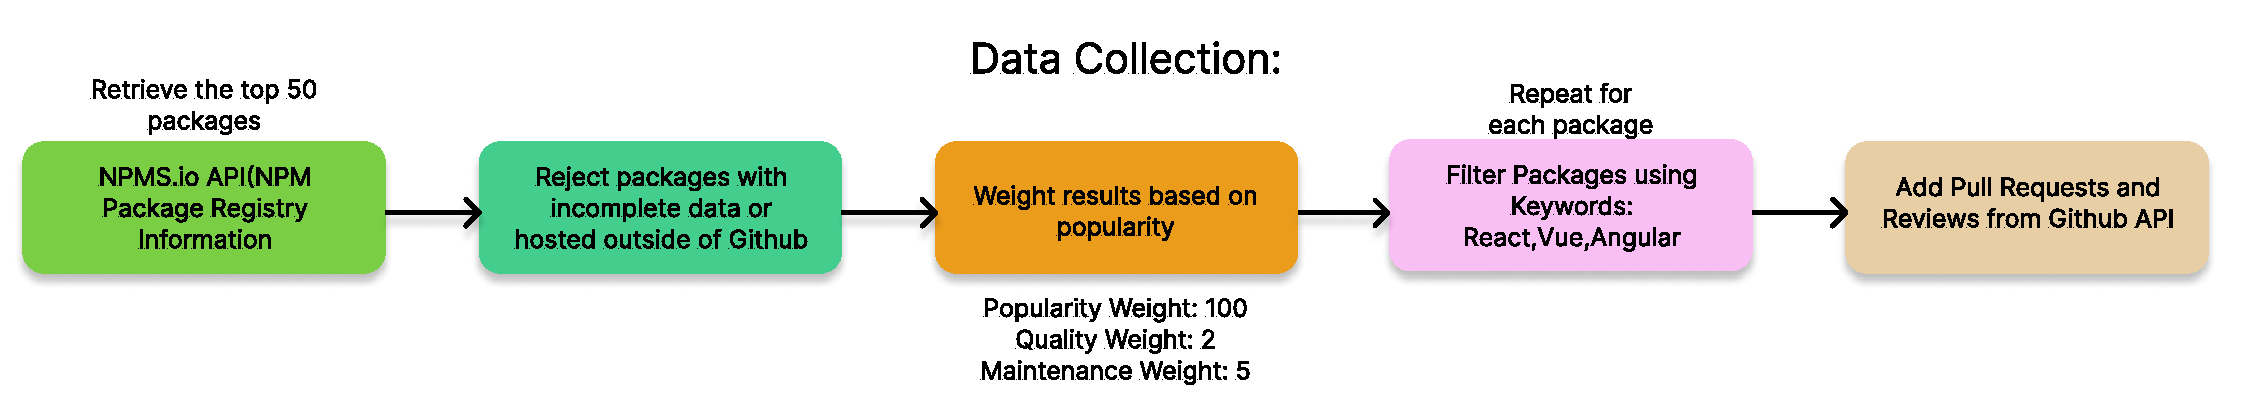
\includegraphics[inner,scale=0.35]{data-collection-flow.pdf}
\caption{Data Collection Pipeline}
\end{figure}



\subsection{Social Network Graph Model}
The Graph Model in this study is simple. The nodes are developers and edges are PR creator to PR reviewer relations.
The graph is unweighted and directed. For each edge, the origin is the creator of the PR in question and the destination is the reviewer. The database diagram(a file-based sqlite database) representing the model above is the following:
\begin{figure}[h]
	\begin{center}
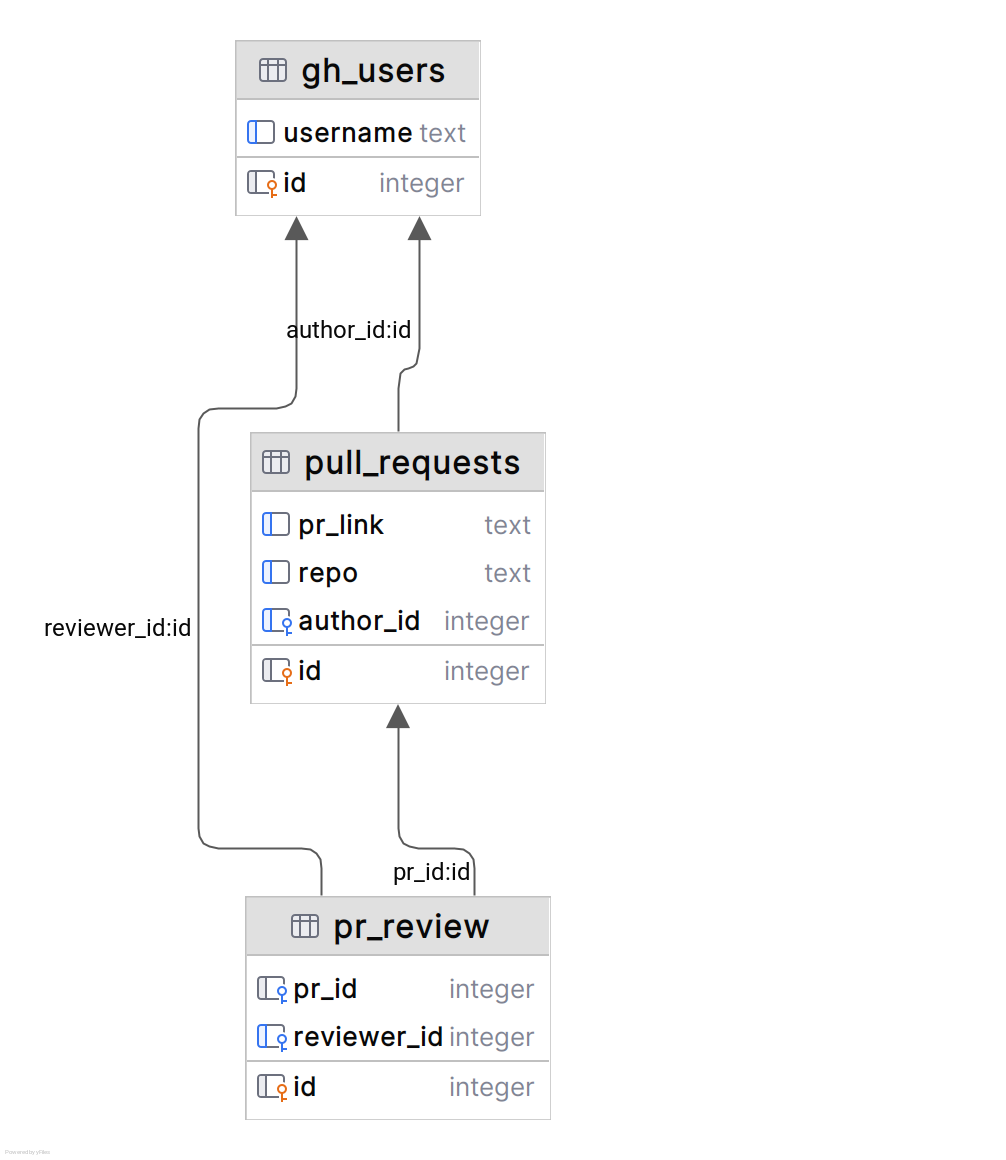
\includegraphics[width=\textwidth,inner,scale=0.5]{code-review-network-db-diagram.png}	
\caption{ER diagram of code review network}
	\end{center}
\end{figure}
\section{Results}
In this context, distance as a general graph metric and shortest distances do not make sense to include in our analysis.
Relevant are the metrics that are centered around node degrees. In this analysis, I focus on degree distributions, degree centralities and scale freeness of the subgraphs created by each package in the dataset.

I define reciprocity as the number of reciprocal edges(divided by two to avoid counting the same reciprocal relation twice). An edge $e_{ij}$ is defined as reciprocal if there exists an edge $e_{ji}$. Percentage reciprocity is thus defined as the number of reciprocal edges divided by the total number of edges.


\begin{figure}[h]
		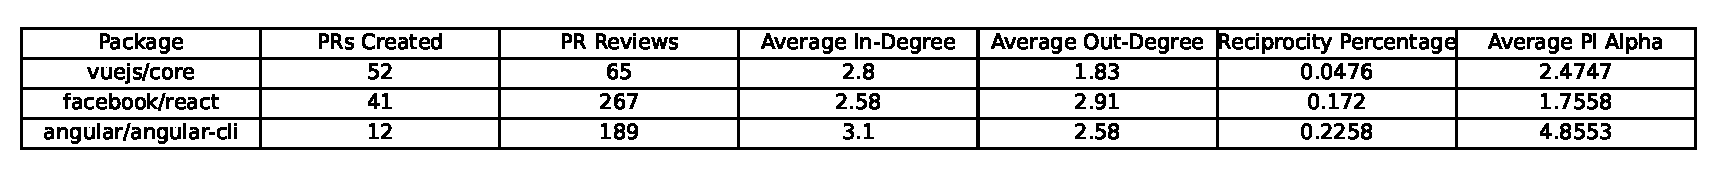
\includegraphics[width=\textwidth,left,scale=1.25]{repo_analysis_table.pdf}	
		\caption{Graph Statistics for the web frontend frameworks introduced}
\end{figure}

Noticeable here is the fact that the $\alpha$ power-law term differs significantly between projects, indicating different development team structures. For Vue, $\alpha \in (2,3)$, for Meta's react $\alpha < 2$ and for angular $\alpha > 3$. A value of $\alpha$ between 2 and 3 indicates scale-free behavior, greater than 3 indicates a heavy tail with fewer hubs and a value less than 2 means an extremely heavy tail.

Degree distributions for each project differ slightly(angular's few PRs retrieved make comparisons meaningless) but have the same structural properties.

\begin{figure}[H]
	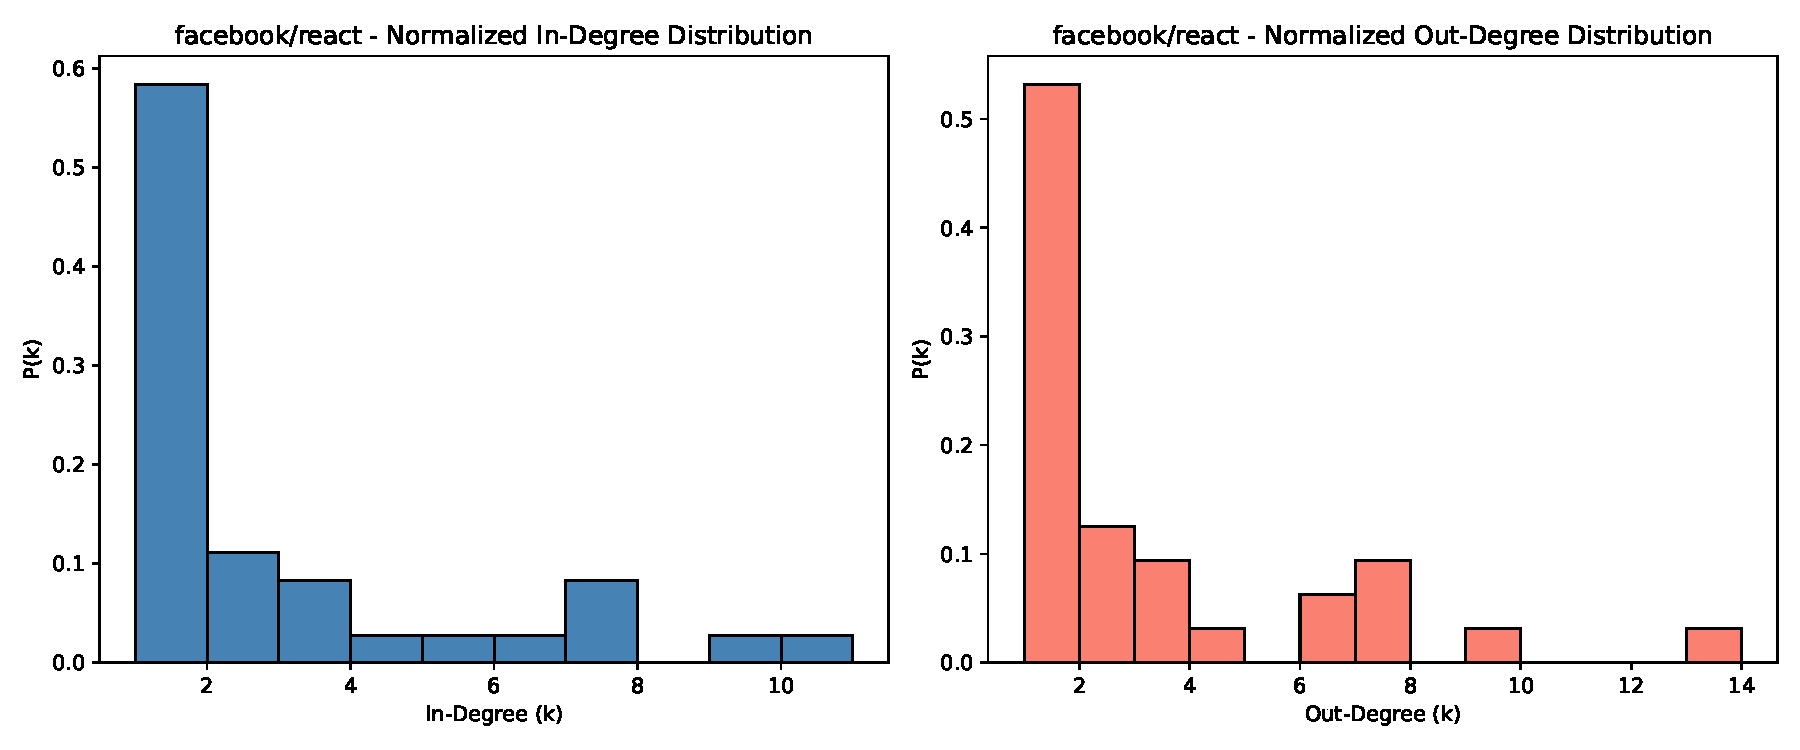
\includegraphics[width=\textwidth,left,scale=1.00]{facebook_react_degree_distribution.pdf}	
	\caption{Degree Distributions for Meta's react}
\end{figure}

\begin{figure}[H]
	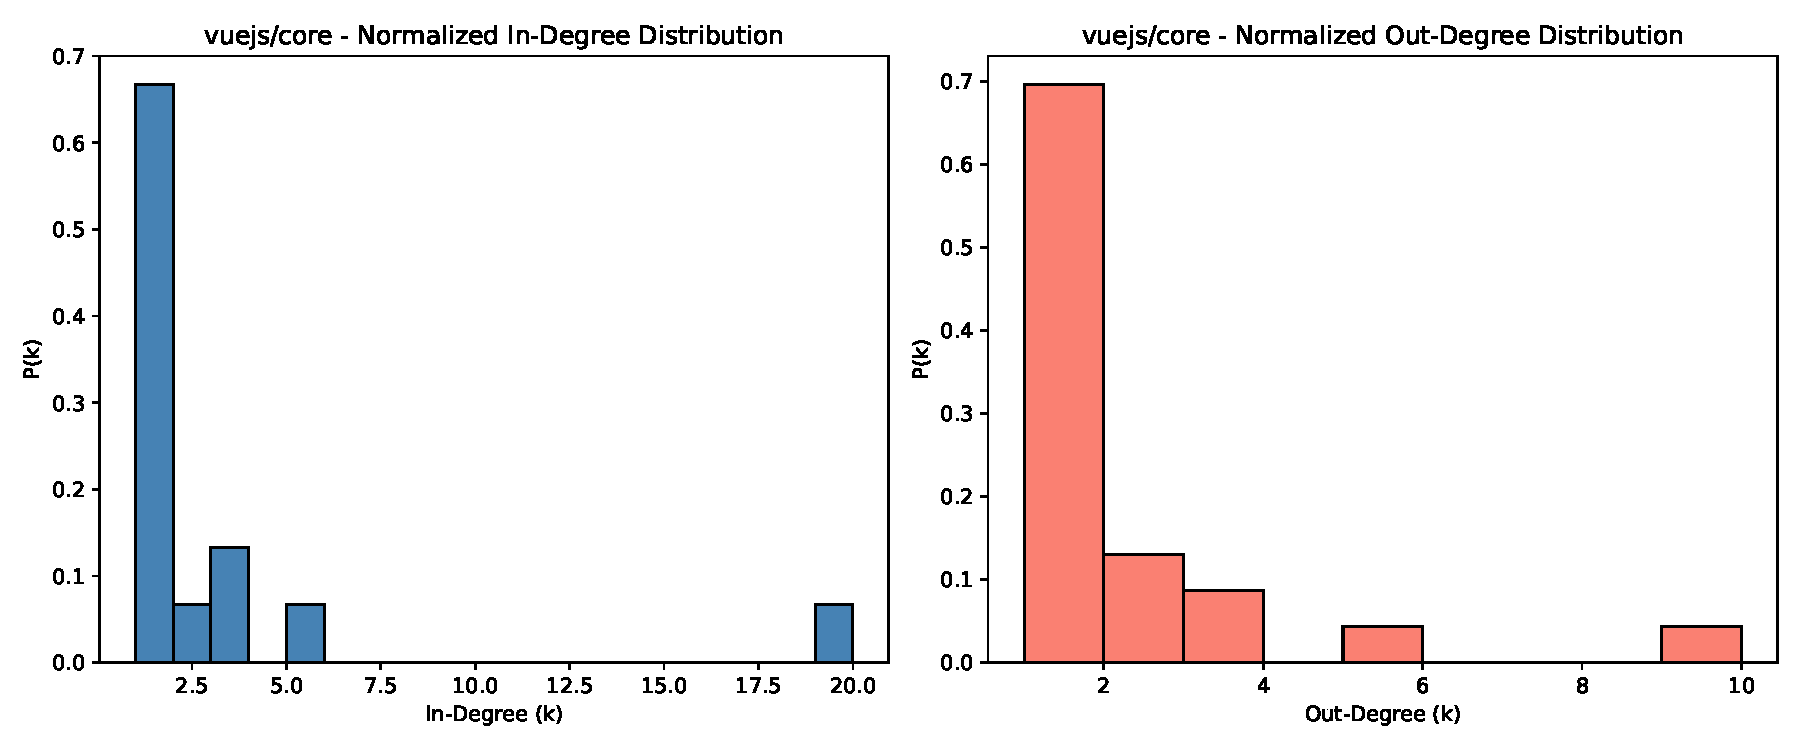
\includegraphics[width=\textwidth,left,scale=1.00]{vuejs_core_degree_distribution.pdf}	
	\caption{Degree Distributions for Vue}
\end{figure}

\begin{figure}[H]
	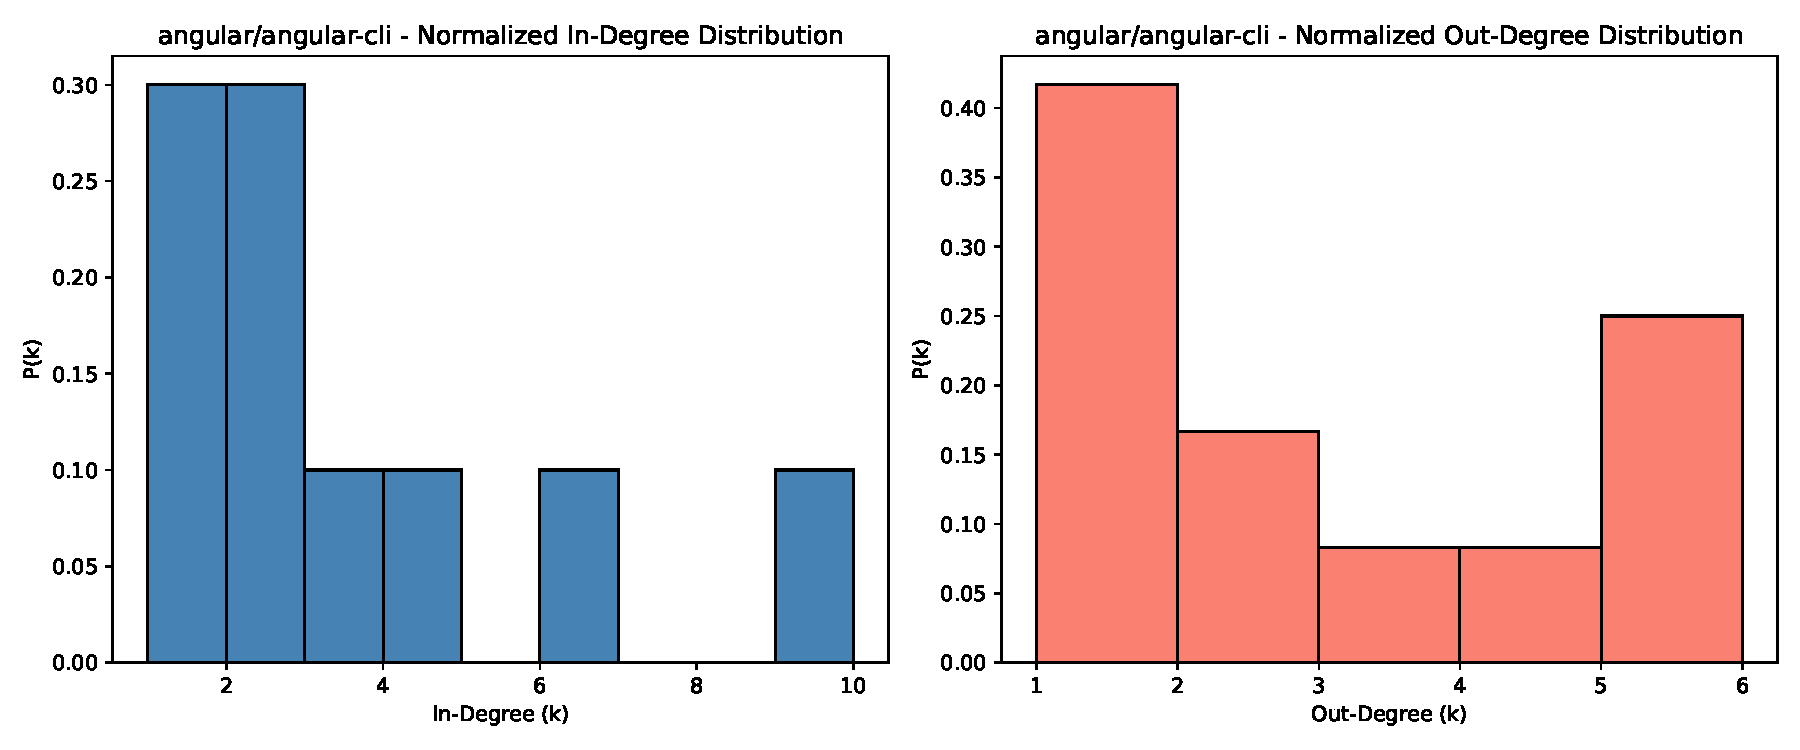
\includegraphics[width=\textwidth,left,scale=1.00]{angular_angular-cli_degree_distribution.pdf}	
	\caption{Degree Distributions for Angular(cli)}
\end{figure}




\section{Conclusion}
As a developer it is important to understand the level of maintenance tooling receives from the community and related companies. Power-law behavior is expected as these pieces of software are extremely complicated and handled by a few experienced professionals involved in the project and occasional third-party contributors. 
An analysis of the underlying code review networks can reveal information on the health of the project, that conventional methods do not usually cover. In this study I attempted to create a simple yet comprehensive dataset to provide the basis of more complex analysis to further understand code review networks and recommend remedies to the pathologies found in such networks.


\bibliography{social-networks}
\bibliographystyle{ieeetr}
\end{document}


